% !TEX encoding = UTF-8 Unicode 
% !TEX root = praca.tex

\chapter{Aplikacja na komputery osobiste}

\section{Wymagania funkcjonalne}

Aplikację zaprojektowano w celu spełnienia następujących wymagań funkcjonalnych:

\begin{itemize}
    \item odczyt próbek sygnału z urządzenia,
    \item wizualizacja sygnału na wykresie w czasie rzeczywistym,
    \item zapis próbek sygnału do pliku.
\end{itemize}


\section{Struktura i środowisko uruchomienia aplikacji}

Na aplikację składają się dwa procesy komunikujące się przy użyciu dostarczonych przez system
operacyjny mechanizmów komunikacji międzyprocesowej:

\begin{itemize}
    \item \textit{serwis} - proces działający w tle, wykrywający podłączone urządzenie, 
    odbierający dane z makiety sprzętowej poprzez odpowiedni sterownik i przekazujący je 
    dalej do \textit{frontendu},

    \item graficzna, okienkowa aplikacja, nazwana krócej \textit{frontendem} - 
     proces odpowiedzialny za wyświetlanie wykresu sygnału odbieranego
    od serwisu i jego zapis do wybranego przez użytkownika pliku.
\end{itemize}

Zarys środowiska w jakim działa aplikacja przedstawiono na diagramie na rys. \ref{fig:app_dpl}.
Procesy \textit{serwisu} oraz \textit{frontendu} są procesami uruchamianymi w przestrzeni użytkownika
(ang. \textit{user space}) systemu \textit{Linux}. \textit{Serwis} komunikuje się przestrzenią 
jądra systemu (ang. \textit{kernel space}) poprzez sterownik 
(w tym wypadku \textit{USB ACM} - będący oficjalną częścią jądra systemu \textit{Linux}), 
który z kolei realizuje komunikację z urządzeniem poprzez fizyczny interfejs. 
Komunikacja ze sterownikiem odbywa się poprzez standardowe wywołania funkcji systemowych (\textit{syscalls}) 
\textit{open}, \textit{close}, \textit{ioctl}, \textit{read} oraz \textit{write}.
Oba programy składające się na aplikację stworzone zostały z zamysłem uruchamiania z poziomu linii poleceń,
umożliwiając wybór różnych opcji i zmianę ich działania poprzez argumenty.

\begin{figure}[h!]
    \centering 
    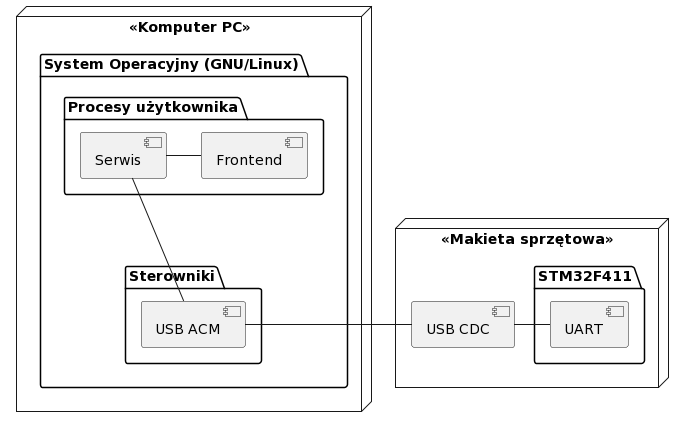
\includegraphics[scale=0.5]{pl/media/deployment.png}
    \caption{Diagram wdrożenia aplikacji}
    \label{fig:app_dpl}
\end{figure}

\newpage

\section{Komunikacja międzyprocesowa}

Do implementacji komunikacji międzyprocesowej użyto mechanizmu \textit{gniazd} 
(\textit{sockets}) zgodnego ze standardem \textit{POSIX.1-2008}.
Procesy uczestniczące w komunikacji podzielono
na dwa typy: serwer i klient. Serwer otwiera \textit{gniazdo} które reprezentowane jest przez
nowo utworzony plik w wirtualnym systemie plików używanym przez system \textit{Linux}. 
Następnie klient otwiera wymieniony plik wirtualny i odczytuje/zapisuje do niego dane za 
pomocą standardowych funkcji \textit{read} 
\footnote{\url{https://man7.org/linux/man-pages/man2/read.2.html}} oraz 
\textit{write} \footnote{\url{https://man7.org/linux/man-pages/man2/write.2.html}}.
W aplikacji w trakcie tworzenia \textit{gniazda} jako argumentu \textit{domain} funkcji
\textit{socket} \footnote{\url{https://man7.org/linux/man-pages/man2/socket.2.html}} 
użyto wartości zdefiniowanej makrem \textit{AF\_UNIX}, natomiast jako argumentu \textit{type}
użyto wartości zdefiniowanej przez \textit{SOCK\_STREAM}. Wymienione wartości argumentów 
ozanaczają że stworzone \textit{gniazdo} służy do dwustronnej, bezstratnej
i niezawodnej komunikacji między procesami.
W aplikacji klientem jest proces \textit{frotnendu}, natomiast serwerem jest proces \textit{serwisu}.
Zatem aby uruchomić \textit{frontend} w celu wyświetlenia lub zapisania sygnału należy na początku
uruchomić proces \textit{serwisu} aby proces \textit{frontendu} mógł się z nim połączyć i zainicjować komunikację.


By zapewnić asynchroniczną i niezawodną komunikację między procesami po obu stronach (klienta i serwera) zastosowano mechanizmy wielowątkowości wraz z odpowiednimi mechanizmami synchronizacji.
W obu przypadkach procesy tworzą dwa wątki: odbierający i wysyłający. Oba te wątki mają dostęp
do współdzielonych z wątkiem głównym buforów typu \textit{FIFO} (\textit{First-In First-Out}).
W przypadku odebrania danych w wątku odbierającym, dane umieszczane są w buforze, 
który następnie może zostać odczytany w wątku głównym. Natomiast w przypadku wątku wysyłającego
to wątek główny zapisuje dane do buforu, które następnie są wysyłane poprzez \textit{gniazdo} w 
wątku wysyłającym. Do rozwiązania klasycznego problemu producenta i konsumenta 
zastosowano w buforach semafory liczące przechowujące liczbę elementów w buforze.
Do stworzenia wątków i ich synchronizacji zastosowano implementacje następujących klas
z biblioteki standardowej języka \textit{C++}: \textit{std::jthread} (tworzenie i kontrola wątków), 
\textit{std::queue} (implementacja buforów), \textit{std::counting\_semaphore} 
(implementacja semaforów). Na rysunku \ref{fig:app_ipc} przedstawiono uproszczony schemat wątków
obu procesów \textit{serwisu} i \textit{frontendu} wraz z buforami.


W celu ujednolicenia interfejsu komunikacyjnego, dane przesyłane między procesami podzielono
na logiczne jednostki, które nazwano pakietami. Każdy pakiet jest traktowany jako łańcuch bajtów
i zawsze zaczyna się bajtem wskazującym typ pakietu a następnie bajtem interpretowanym jako liczba
w naturalnym kodzie binarnym, reprezentująca długość całego pakietu w bajtach. Reszta pakietu
zawiera dane specyficzne dla typu pakietu.\\ 
Dla czytelności bajty pakietów oznaczono następującą notacją: 

- $[i]$ reprezentuje $i$-ty bajt w łańcuchu, dla $i \in [0, N-1]$ gdzie $N$ to długość pakietu,

- $[a:b]$ reprezentuje łańcuch bajtów $[a]$, $[a+1]$, $...$, $[b-1]$, $[b]$. 

Typy pakietów wraz z opisem zawarto w tabeli \ref{tab:ipc_types}.

\begin{table}[h!]
\centering
    \caption{Typy pakietów (zapisane w systemie szesnastkowym)
    użyte w komunikacji \\międzyprocesowej w aplikacji}
\label{tab:ipc_types}
\begin{tabular}{|l|l|lll}
\cline{1-2}
$[0]_{16}$ & \textit{Opis}             &  &  &  \\ \cline{1-2}
00 & Próbka sygnału                         &  &  &  \\ \cline{1-2}
03 & Żądanie rozpoczęcia przesyłania próbek &  &  &  \\ \cline{1-2}
04 & Żądanie zatrzymania przesyłania próbek &  &  &  \\ \cline{1-2}
05 & Potwierdzenie wykonania żądania        &  &  &  \\ \cline{1-2}
80 & Błąd: nieprawidłowy pakiet             &  &  &  \\ \cline{1-2}
83 & Błąd: już rozpoczęto przesyłanie próbek&  &  &  \\ \cline{1-2}
85 & Błąd: urządzenie niepodłączone         &  &  &  \\ \cline{1-2}
\end{tabular}
\end{table}

Pakiety o wartościach $03-05$ i $80-85$ mają długość $N=2$ i nie zawierają dodatkowych 
bajtów poza bajtami typu i długością.
Natomiast struktura całego pakietu reprezentującego próbkę sygnału przedstawiona została w tabeli
\ref{tab:ipc_sample_pack}. Bajty $[2:5]$ oznaczające numer próbki interpretowane są jako 32-bitowa
liczba całkowita zapisana w naturalnym kodzie binarnym, 
natomiast wartość próbki jest interpretowana jako liczba zmiennoprzecinkowa pojedynczej precyzji w standardzie \textit{IEEE 754} \cite{IEE754}.

\begin{table}[h!]
\centering
\caption{Struktura pakietu zawierającego próbkę sygnału}
\label{tab:ipc_sample_pack}
\begin{tabular}{|l|l|l|l|}
\hline
$[0]$       & $[1]$           & $[2:5]$      & $[6:9]$        \\ \hline
Typ pakietu & Rozmiar pakietu & Numer próbki & Wartość próbki \\ \hline
\end{tabular}
\end{table}

\newpage

Typowy przypadek komunikacji między dwoma procesami w aplikacji wygląda następująco:

1. Serwer tworzy i otwiera \textit{gniazdo}.

2. Klient łączy się z serwerem i wysyła pakiet z żądaniem rozpoczęcia przesyłania próbek.

3. Jeżeli makieta sprzętowa jest podłączona serwer odpowiada potwierdzeniem wykonania żądania,
w przeciwnym wypadku przesyłany jest pakiet o typie $85$ (tabela \ref{tab:ipc_types}).

4. Po potwierdzeniu wykonania żądania, serwer zaczyna przesyłać pakiety z próbkami sygnału odczytanego z makiety sprzętowej.

Przykład komunikacji między między procesami w aplikacji przedstawiono również na rysunku \ref{fig:ipc_seq}.

\begin{figure}[h!]
    \centering 
    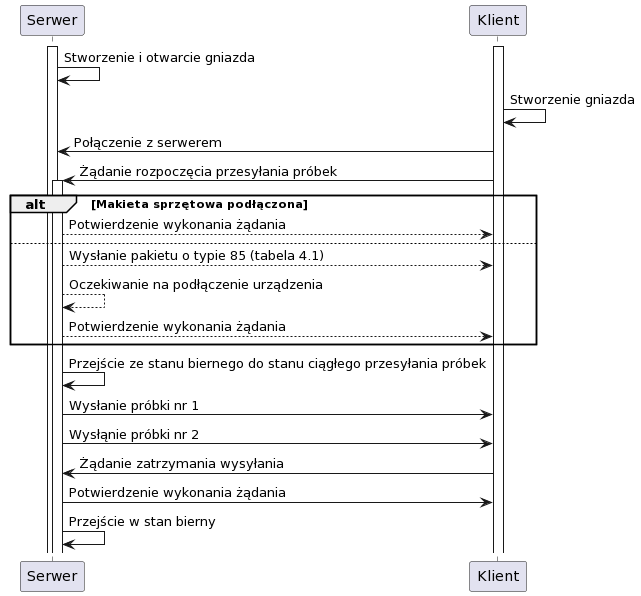
\includegraphics[scale=0.75]{pl/media/ipc_sequence.png}
    \caption{Diagram sekwencji dla przykładowego przebiegu komunikacji między klientem a serwerem (w kontekście aplikacji: 
    \textit{frontendem} a \textit{serwisem})}
    \label{fig:ipc_seq}
\end{figure}

\newpage

\section{Serwis}

Podobnie jak \textit{frontend}, \textit{serwis} posiada dwa wątki do komunikacji międzyprocesowej.
Program ten tworzy również dwa dodatkowe wątki: odpowiadający za wykrywanie i otwarcie urządzenia jeśli jest podłączone
oraz wątek odczytujący dane z urządzenia.
Proces serwisu uruchamiany jest z argumentami z linii poleceń wybranej przez użytkownika powłoki
(\textit{shell}). Możliwe opcje i wartości argumentów wraz z wyjaśnieniem przedstawiono tabeli \ref{tab:daemon-cmd-args}.

\begin{table}[h!]
\centering
    \caption{Argumenty linii poleceń \textit{serwisu} wraz z opisami}
\label{tab:daemon-cmd-args}
    \begin{tabular}{|p{0.18\linewidth}|p{0.4\linewidth}|p{0.42\linewidth}|}
\hline
    \textbf{Argument} & \textbf{Parametr} & \textbf{Opis}        \\ \hline
    \textit{-h} & - & Wypisanie tekstu pomocniczego (\textit{help}) opisującego argumenty.\\ \hline
    \textit{-v} & - & Włączenie wypisywania szczegółowych komunikatów na standardowe wyjście.   \\ \hline
    \textit{-s} & - & Wyłączenie wypisywania komunikatów (poza błędami) na standardowe wyjście. \\ \hline
    \textit{--frontend-sockn} & Ścieżka do tworzonego gniazda. & Użycie niedomyślnej ścieżki do gniazda tworzonego przez \textit{serwis} dla procesu \textit{frontendu}. \\ \hline
    \textit{--wired} & Ścieżka do pliku wirtualnego urządzenia. & Użycie pliku wirtualnego o podanej ścieżce do komunikacji z makietą sprzętową. \\ \hline
\end{tabular}
\end{table}

Przykładowe wywołanie i komunikaty z linii poleceń uruchomionego serwisu przedstawiono na listingu \ref{listing:ecgmd}.
W pierwszej linii listingu \ref{listing:ecgmd} przedstawiono przykładowy sposób uruchomienia programu wraz z przykładowymi
argumentami: program uruchomiono z dodatkową opcją \textit{-v} (tabela \ref{tab:daemon-cmd-args}) i ścieżką do pliku wirtualnego
odpowiadającego urządzeniu makiety sprzętowej. Następnie wypisywane są komunikaty mówiące o oczekiwaniu serwisu na połączenie
się z procesem \textit{frontendu} jak i z urządzeniem.

\begin{listing}
\begin{minted}{text}
./ecgmd -v --wired /dev/serial/by-id/usb-STMicroelectronics_STM32_STLink_(...)
[00:42:25][status] 	Waiting for device to connect ...
[00:41:25][status] 	Waiting for the frontend to connect...
\end{minted}
    \caption{Przykładowe wywołanie programu serwisu aplikacji}
\label{listing:ecgmd}
\end{listing}

Serwis wspiera również tzw. \textit{hot plugging} urządzenia. Urządzenie jest stale
monitorowane przez dodatkowy wątek, który w wypadku wykrycia odłączenia zatrzymuje próby odczytu danych.
Program nie zamyka się ani nie zgłasza błędu, po ponownym podłączeniu rozpoczyna na nowo odbieranie
próbek oraz ich przesyłanie do \textit{frontendu}.

\newpage

\section{Frontend}

Poza dwoma wątkami biorącymi udział w komunikacji międzyprocesowej oraz wątkiem głównym, 
podczas uruchomienia proces \textit{frontendu} tworzy jeszcze dodatkowo wątek rysujący
(rys. \ref{fig:app_ipc}; wątek rysujący jest tworzony wyłącznie w przypadku braku argumentu \textit{--nographic}, tabela \ref{tab:frontend-cmd-args}). Wątek rysujący używa biblioteki \textit{SDL2} do wyświetlania dynamicznej grafiki rastrowej, do otwarcia
okna oraz obsługi wejścia od myszki i klawiatury. 

\begin{listing}
\begin{minted}{c++}
class observer
{
public:
    virtual void notify(void*) = 0;
};
\end{minted}
    \caption{Interfejs obserwatora}
\label{listing:observer}
\end{listing}

W implementacji klasy rysującej wykres oraz klasy odpowiadającej za zapis sygnału do pliku użyto wzorca obserwatora 
(ang. \textit{Observer}, interfejs przedstawiony na listingu \ref{listing:observer}) - powszechnie znanego wzorca projektowego. 
W przypadku odebrania przez wątek główny próbek sygnału
klasa rysująca oraz klasa zapisująca sygnał otrzymują powiadomienia poprzez metodę \textit{notify} wywołaną w wątku głównym 
z argumentem będącym indeksem, wskazującym na numer próbki która została dodana do globalnego bufora.
W wątku głównym przechowywane są jedynie wskaźniki na obiekty implementujące interfejs \textit{observer} co pozawala w chwili
potrzeby przerysowania wykresu (lub jego fragmentu) lub zapisu do pliku, wywołać na nich po kolei metodę \textit{notify}.

\begin{table}[h!]
\centering
    \caption{Argumenty linii poleceń \textit{frontendu} wraz z opisami}
\label{tab:frontend-cmd-args}
    \begin{tabular}{|p{0.18\linewidth}|p{0.4\linewidth}|p{0.42\linewidth}|}
\hline
    \textbf{Argument} & \textbf{Parametr} & \textbf{Opis}        \\ \hline
    \textit{-h} & - & Wypisanie tekstu pomocniczego (\textit{help}) opisującego argumenty.\\ \hline
    \textit{-v} & - & Włączenie wypisywania szczegółowych komunikatów na standardowe wyjście.   \\ \hline
    \textit{-s} & - & Wyłączenie wypisywania komunikatów (poza błędami) na standardowe wyjście. \\ \hline
    \textit{--sockn} & Ścieżka do gniazda \textit{serwisu}. & Użycie niedomyślnej ścieżki do gniazda \textit{serwisu}. \\ \hline
    \textit{--file} & Ścieżka do pliku tekstowego. & Włączenie zapisu próbek sygnału do wybranego pliku tekstowego. \\ \hline
    \textit{--nographic} / \textit{-ng} & - & Wyłączenie wyświetlania wykresu sygnału w czasie rzeczywistym. \\ \hline
\end{tabular}
\end{table}

\newpage

\begin{figure}[h!]
    \centering 
    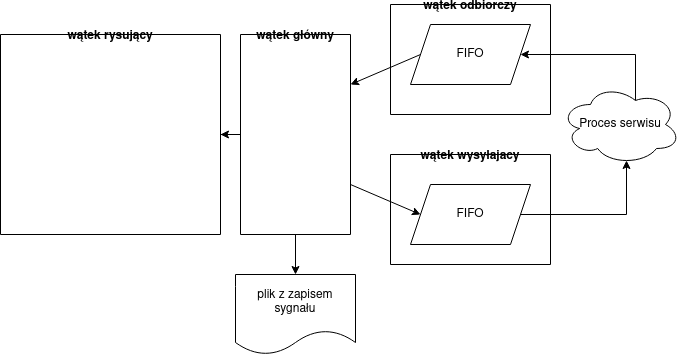
\includegraphics[scale=0.5]{pl/media/app_ipc.png}
    \caption{Rysunek poglądowy przedstawiający strukturę wątków dla procesu \textit{frontendu}}
    \label{fig:app_ipc}
\end{figure}

\begin{figure}[h!]
    \centering 
    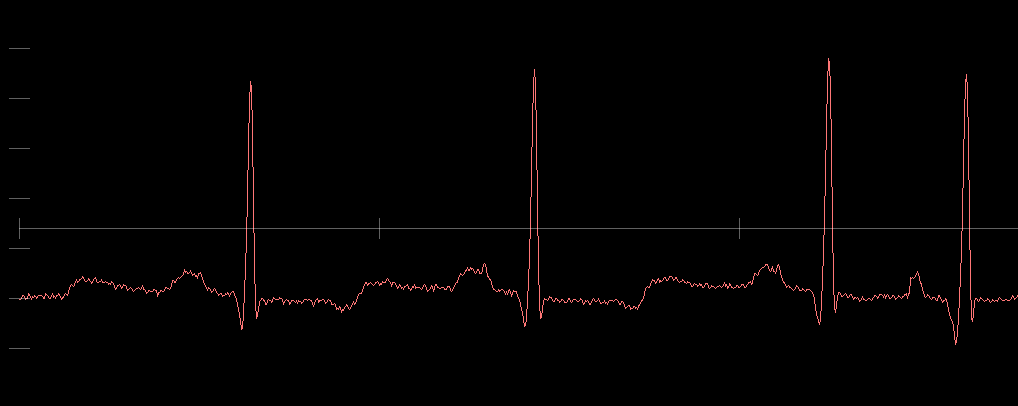
\includegraphics[scale=0.45]{pl/media/frontend_window.png}
    \caption{Zrzut ekranu przedstawiający okno \textit{frontendu} z wykresem sygnału EKG 
    (w trybie graficznym, tzn. bez argumentu \textit{--nographic})}
    \label{fig:frontendwin}
\end{figure}

Przykładowe uruchomienie programu \textit{frontendu} przedstawiono na listingu \ref{listing:ecgmapprun}.
W pierwszej linii przedstawiono przykładowy sposób uruchomienia programu wraz z przykładowymi argumentami.
W przykładzie z listingu \ref{listing:ecgmapprun} \textit{frontend} uruchomiony został w trybie bez
okienka wykresu sygnału, z zapisem do pliku \textit{signal.txt}. Zapisywany do pliku sygnał ma
postać listy liczb rzeczywistych zapisanych w postaci tekstowej, oddzielanych znakiem nowej linii.

\begin{listing}
\begin{minted}{text}
./ecgm_app  --file singal.txt --nographic 
[19:50:18][status] 	Trying to connect to a ecgmd service...
[19:50:18][status] 	Connected.
[19:50:18][status] 	ACK received, the device is running.
\end{minted}
    \caption{Przykładowe wywołanie \textit{frontendu} aplikacji}
\label{listing:ecgmapprun}
\end{listing}

\newpage

\section{Kompilacja i uruchomienie}

Wymagania odnośnie środowiska kompilacji:

- system operacyjny \textit{GNU/Linux} (aplikacja przetestowana na wersji \textit{6.6.9}),

- kompilatory i narzędzia do konsolidacji dla języka \textit{C++20}
  (preferowany kompilator z kolekcji \textit{GCC}, w wersji: \textit{13.2.1}),

- biblioteka SDL w wersji 2.0 lub wyższej,

- programy CMake (wersja: 3.20 lub wyższa) oraz GNU Make (4.4.0 lub wyższa),

- powłoka systemowa np. \textit{bash} lub \textit{zsh}

Na listingu \ref{listing:buildinst} przedstawiono komendy powłoki jakie należy wykonać w celu prawidłowego
zbudowania aplikacji. Poniższy listing zakłada, że na początku katalog roboczy użytkownika to katalog 
nadrzędny w drzewie katalogów zawierających kod źródłowy aplikacji.

\begin{listing}
\begin{minted}{bash}
mkdir build && cd build
cmake .. && make
\end{minted}
    \caption{Kroki budowania aplikacji}
\label{listing:buildinst}
\end{listing}

W celu uruchomienia aplikacji należy użyć dwóch instancji powłoki, w jednej z nich na początku uruchomić program
\textit{ecgmd} (\textit{serwis}), znajdujący się w katalogu \textit{./services/ecgmd/}.
Po uruchomieniu \textit{serwisu} możliwe jest uruchomienie programu \textit{ecgmd\_app} (\textit{frontendu}), znajdującego
się w bieżącym katalogu. Dla ułatwienia uruchamiania całości aplikacji stworzony został 
skrypt w języku \textit{bash} umożliwiający szybkie i łatwe uruchomienie obu procesów aplikacji, 
zawartość skryptu przedstawiono na listingu \ref{listing:runscript}.

\begin{listing}
\begin{minted}{bash}
#!/bin/bash
DEV=\
'/dev/serial/by-id/usb-STMicroelectronics_STM32_STLink_066DFF383638534B43224635-if02'

if [[ $? -eq 2 ]] then
    DEV=$1 
fi
echo "Using device path: $DEV"

./build/services/ecgmd/ecgmd -v --wired $DEV > ecgmd.log &
sleep 1
./build/ecgm_app > app.log &
wait
\end{minted}
    \caption{Skrypt uruchamiający całą aplikację.}
\label{listing:runscript}
\end{listing}
